%---------------------------------------------
%
%       START
%
%---------------------------------------------

\chapter{Supplementary data to \Chapref{TEM_paper}}
%\chapter{Supplementary Information to \Chapref{Longevity}}%labstudy is the label for chapter 2.
\label{chap:Appendix_TEM_paper}

\bigskip
\medskip
\begin{center}

\noindent{\Large \bf  Effects of missing data on topological inference using a Total Evidence approach} \\
\bigskip
\end{center}

The following section contains supplementary results to the chapter ``Effects of missing data on topological inference using a Total Evidence approach''.

\section{Differences between the ``true'' and the inferred trees.}

In our simulation protocol, we used the ``true'' tree to generate the molecular characters and the morphological characters for the living and fossil taxa (i.e. the ``complete'' matrix).
Therefore, the ``true'' tree can be seen as a random seed for starting our simulations.
The following analysis measures the performance of our parameter and algorithms choices to generate the ``complete'' matrix.
To asses the performance of our simulation protocol, we compared our ``true'' trees (i.e. the trees \textbf{used to create} the ``complete'' matrices) to the ``best'' trees (i.e. the trees \textbf{inferred from} the ``complete'' matrices; Fig. ~\ref{Fig_Supp_True_Best}).
Note that the difference between the ``true'' and the ``best'' trees represents the effect of the parameters choice and the algorithms used to create the ``complete'' matrix as well the as the capacity of RAxML and MrBayes to infer phylogenies from this particular matrices (i.e. small sized and generated using specific algorithms).
This does not affect, however, the results of our analysis since we deliberately compared the the ``missing-data'' trees to the ``best'' tree rather than to the ``true'' tree. 

\begin{figure}%[!ht]
\centering
    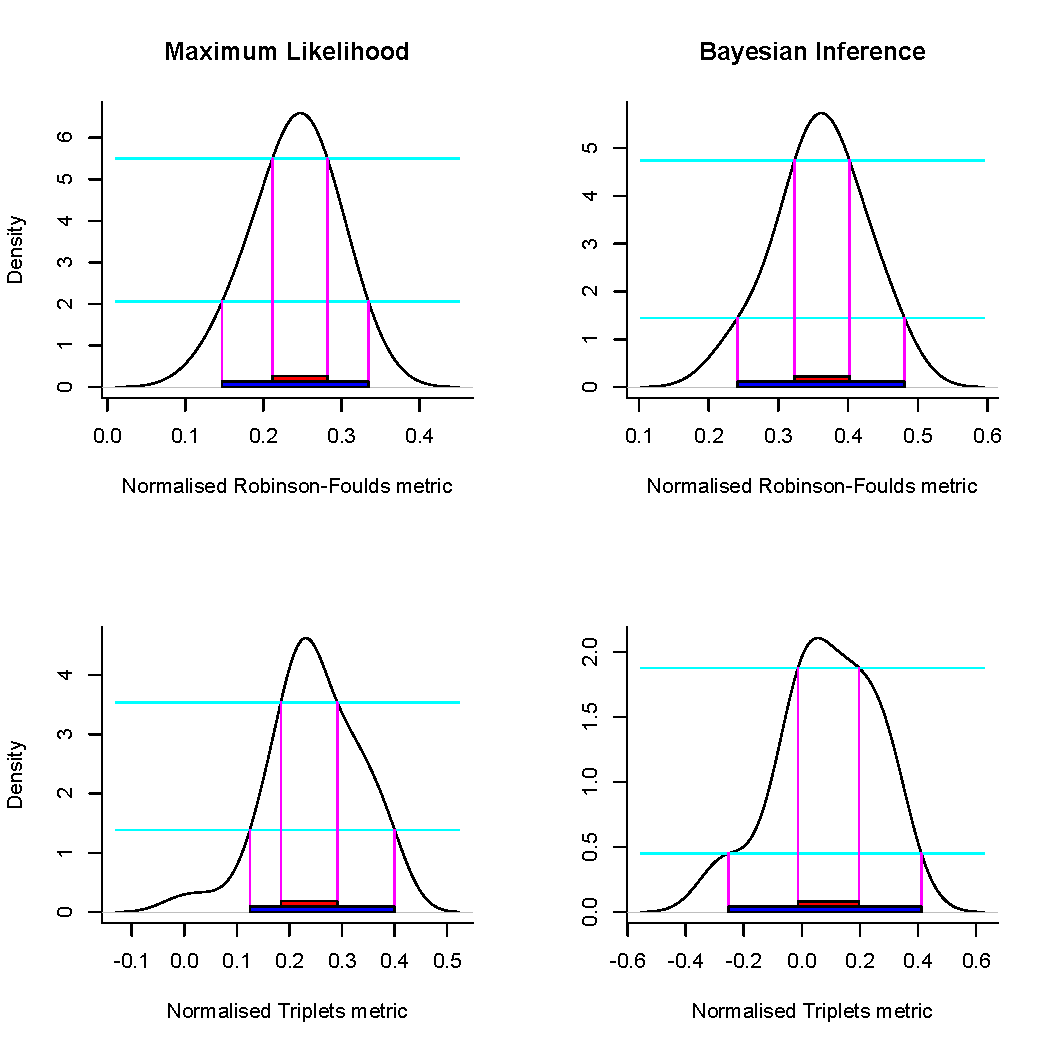
\includegraphics[width=1\textwidth]{Supplementaries/Figures/TEM/True_vs_Best_trees.pdf}
    \caption[Comparison between the ``true'' and the ``best'' trees]{Pairwise comparisons among the 50 ``true'' trees and the 50 ``best'' trees from the Maximum Likelihood and Bayesian inference methods. The horizontal blue and red lines represent, respectively, the 95\% and 50\% confidence intervals.} 
\label{Fig_Supp_True_Best} 
\end{figure}

\begin{figure}%[!ht]
\centering
    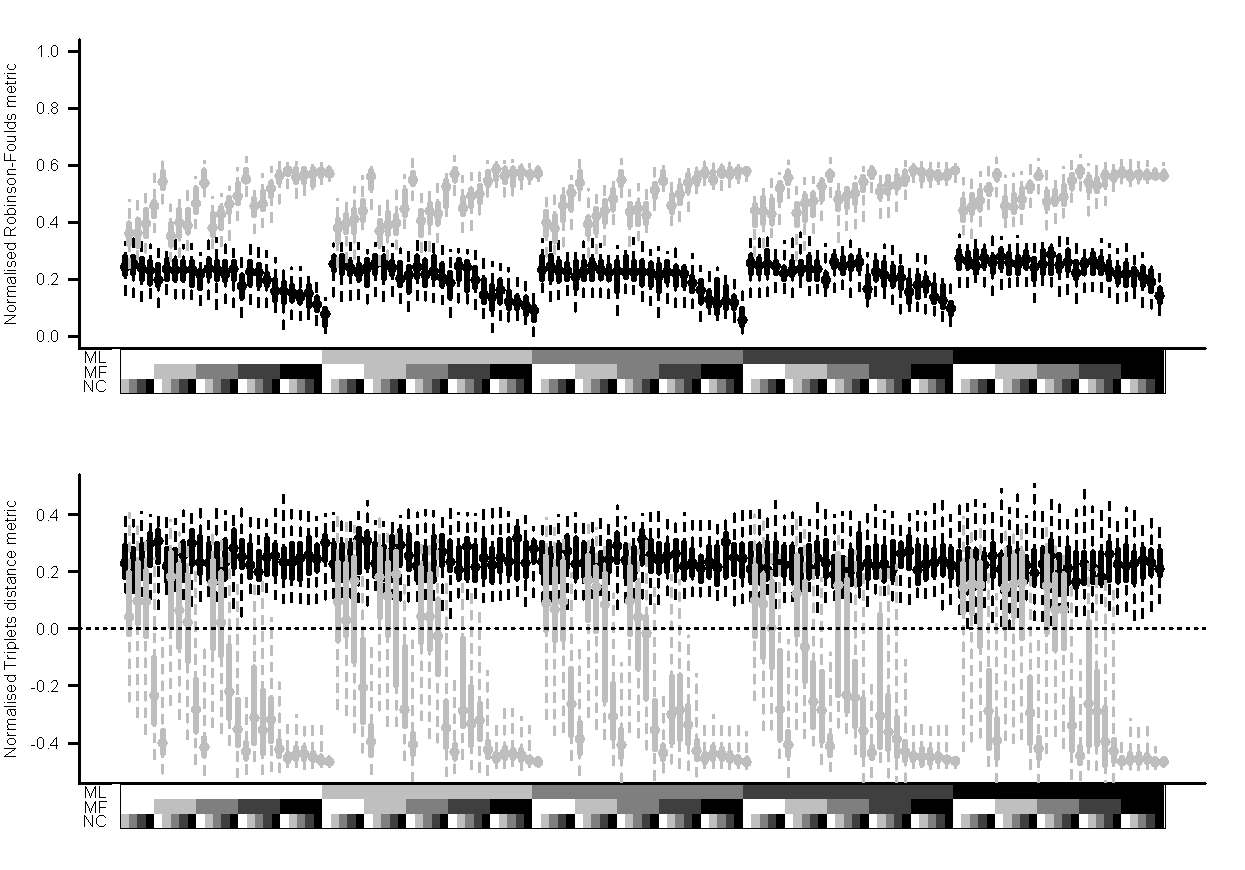
\includegraphics[width=1\textwidth]{Supplementaries/Figures/TEM/Singles_True.pdf}
    \caption[Comparison between the ``true'' and the ``missing-data'' trees for the Maximum Likelihood an Bayesian consensus trees]{Effect of increasing missing data on recovering the ``true'' tree topology (the tree used for starting our simulations) for the Maximum Likelihood trees (black) and Bayesian consensus trees (grey). The x axis shows the percentage of missing data from 0\% (white) to 75\% (black) for the two parameters: $M_{L}$ (upper line), $M_{F}$ (middle line) and number of characters from 100 to 25 for the parameter $N_{C}$ (lower line). Topological recovery was measured using two different tree comparison metrics: Normalised Robinson-Foulds metric (upper row) and Normalised Triplets metric (lower row). The graph shows the modal value (points), and the 50\% (thick solid lines) and 95\% (thin dashed lines) confidence intervals of the distributions of the tree comparison metric for each missing data parameter and tree inference method.} 
\label{Fig_Supp_Singles_true} 
\end{figure}

\begin{figure}%[!ht]
\centering
    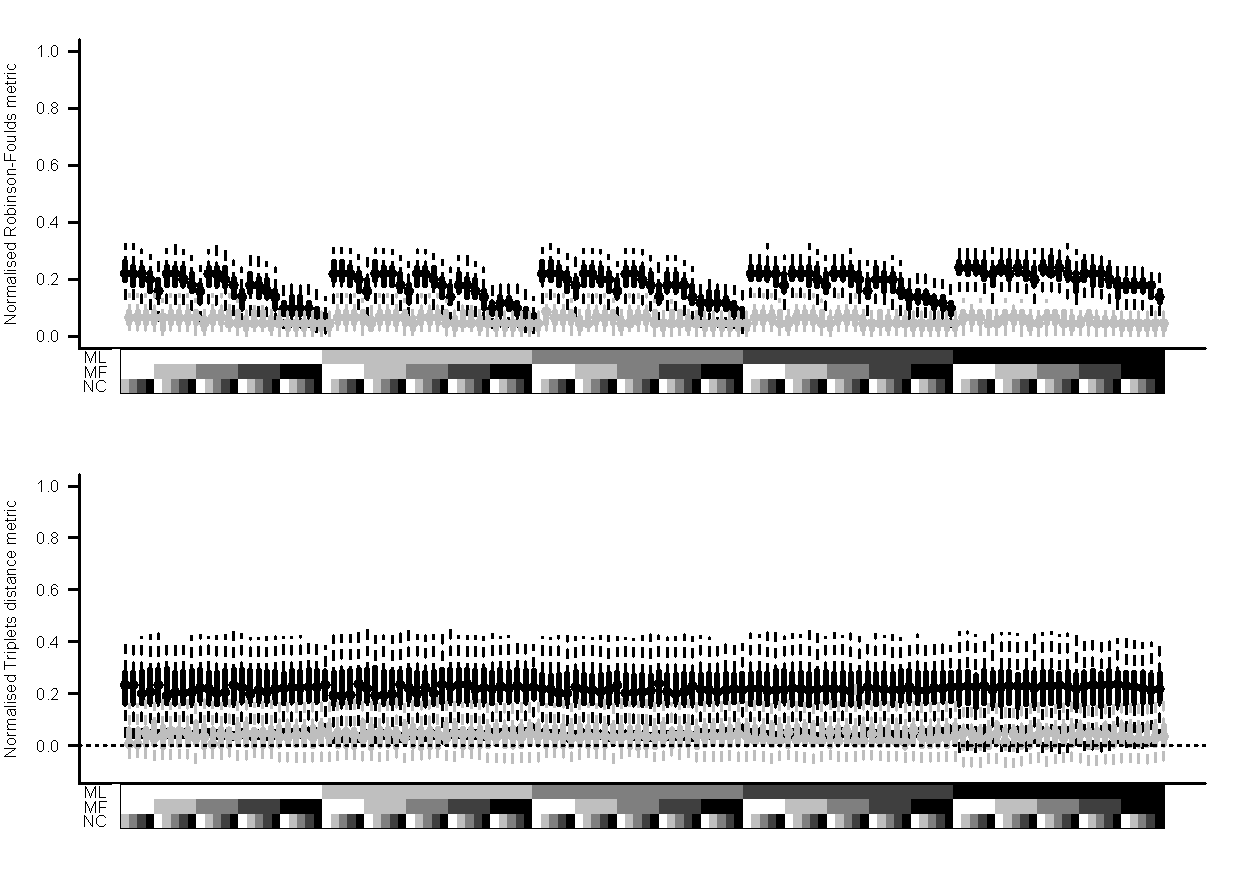
\includegraphics[width=1\textwidth]{Supplementaries/Figures/TEM/Treesets_True.pdf}
    \caption[Comparison between the ``true'' and the ``missing-data'' trees for the Bootstraps and posterior distribution trees]{Effect of increasing missing data on topological recovering the ``true'' tree topology (the tree used for starting our simulations) for the Maximum Likelihood Bootstrap trees (black) and Bayesian posterior tree distribution (grey). The x axis shows the percentage of missing data from 0\% (white) to 75\% (black) for the two parameters: $M_{L}$ (upper line), $M_{F}$ (middle line) and number of characters from 100 to 25 for the parameter $N_{C}$ (lower line). Topological recovery was measured using two different tree comparison metrics: Normalised Robinson-Foulds metric (upper row) and Normalised Triplets metric (lower row). The graph shows the modal value (points), and the 50\% (thick solid lines) and 95\% (thin dashed lines) confidence intervals of the distributions of the tree comparison metric for each missing data parameter and tree inference method.} 
\label{Fig_Supp_Treesets_true} 
\end{figure}

\newpage
\section{Tree Inference Software settings}

For clarity we have provided the exact settings used in our tree building below.
\subsection*{Maximum Likelihood: RAxML version 8.0.20 \cite{Stamatakis21012014}}
\begin{itemize}
  \item Molecular data: GTR + $\Gamma_4$ (-m GTRGAMMA)
  \item Morphological data: M\textit{kv} + $\Gamma_4$ (-K MK)
  \item Support: Rapid Boostrap algorithm (LSR), 1000 replicates
\end{itemize}
\subsection*{Bayesian: MrBayes version 3.2.1 \cite{Ronquist2012mrbayes}}
\begin{itemize}
  \item Priors: Molecular data
  \begin{itemize}
    \item Rates distribution shape ($\alpha$) = 0.5
    \item Transition/Transversion ratio = 2 ($\beta$(80,40))
    \item Starting tree: "True" tree topology with each branch length = 1
  \end{itemize}
  \item Priors: Morphological data
  \begin{itemize}
    \item rates distribution shape ($\alpha$) = 0.5
  \end{itemize}
  \item Models
  \begin{itemize}
    \item Molecular data: HKY + $\Gamma_4$
    \item Morphological data: M\textit{kv} + $\Gamma_4$
  \end{itemize}
  \item MCMC
  \begin{itemize}
    \item Two runs
    \item Four chains per run
    \item Generations $<$ $5$$\times$$10^7$
    \item Sample frequency = $1.05$$\times$$10^4$
    \item ASDS diagnosis frequency = $5$$\times$$1^4$
    \item ASDS $<$ 0.01
    \item ESS $>>$ 200
    \item Burnin = 25\%
  \end{itemize}
\end{itemize}